\section{Results}
\label{sec:results}

In the following, we report and analyze the results of the experiments described in the previous section. 

\subsection{Representation Modules}

\subsubsection{Decoder Output}
We begin by qualitatively analyzing the reconstructions created by the variational autoencoder (VAE), the Janus architecture and the Cerberus architecture. Note that while we will loosely refer to the outputs of the decoders as \textit{reconstructions} in the following, only the leftmost output of the multi-decoder architectures is an actual reconstruction. As described in Section \ref{sec:approach}, the middle and right output are predictions or approximations of unseen information.

\begin{figure}[t!]
	\centering
	\begin{subfigure}{0.6\columnwidth}
		\centering
		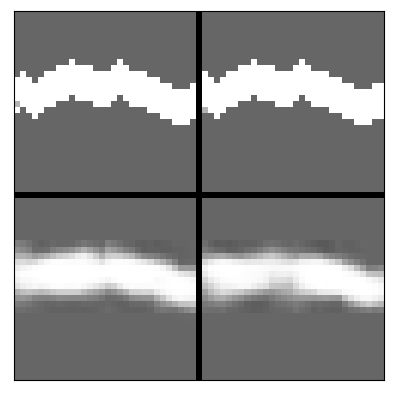
\includegraphics[width=\linewidth]{img/janus_tunnel_recon.png}
		\caption{Janus. Left is the current frame, right is the next frame.}
		\label{subfig:janus_reconstruction}
	\end{subfigure}%
	~ 
	\begin{subfigure}{0.3\columnwidth}
		\centering
		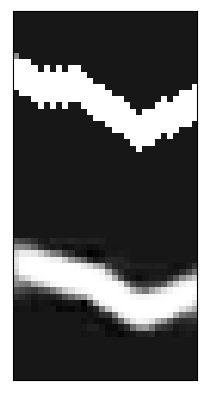
\includegraphics[width=\linewidth]{img/cvae_tunnel_recon.png}
		\caption{CVAE.}
		\label{subfig:cvae_reconstruction}
	\end{subfigure}
	
	
	\begin{subfigure}{0.9\columnwidth}
		\centering
		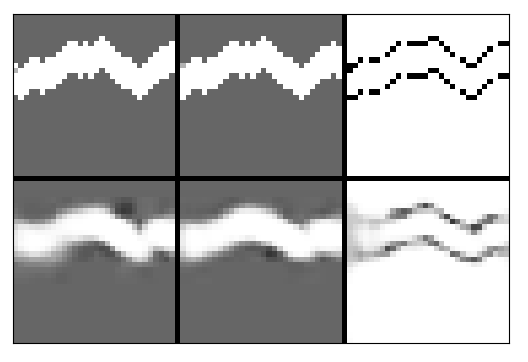
\includegraphics[width=\linewidth]{img/cerberus_tunnel_recon.png}
		\caption{Cerberus. From left to right are the current frame, next frame, and the differences between the two frames.}
		\label{subfig:cerberus_reconstruction}
	\end{subfigure}

	\caption{Reconstruction of the different representation learners performing over the Tunnel task. For each architecture the ground-truth (upper images) and the reconstructions (lower images) are depicted.}
	\label{fig:repr_learner_reconstructions}
\end{figure}

Figures \ref{fig:repr_learner_reconstructions} to \ref{fig:cvae_multitask} show examples of the outputs of the decoders in the three different architectures. Figure \ref{fig:repr_learner_reconstructions} is the result of 500,000 episodes of training on the Tunnel task. It comes unsurprising that the reconstructions are not perfect, since the environment is randomly generated. Out of the three architectures, Janus seems to be most flawed. Although the course of the tunnel seems correctly reconstructed, its borders are a lot blurrier. The CVAE appears to reconstruct slightly more defined borders and also approximates the tunnel's course well. Similarly, Cerberus produces borders that are more clearly defined than in Janus.

% CVAE MT
\begin{figure}[t!]
	\centering
	\begin{subfigure}{0.3\columnwidth}
		\centering
		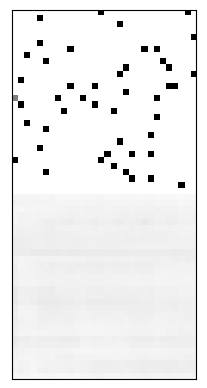
\includegraphics[width=\linewidth]{documentation/report/img/cvae_scroll_evasion.png}
		\caption{Evasion.}
		\label{subfig:cvae_scroll_race}
	\end{subfigure}%
	~ 
	\begin{subfigure}{0.3\columnwidth}
		\centering
		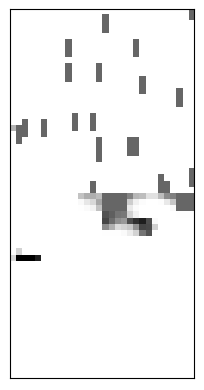
\includegraphics[width=\linewidth]{documentation/report/img/cvae_scroll_walls.png}
		\caption{Wall Evasion.}
		\label{subfig:cvae_scroll_walls}
	\end{subfigure}
	~ 
	\begin{subfigure}{0.3\columnwidth}
		\centering
		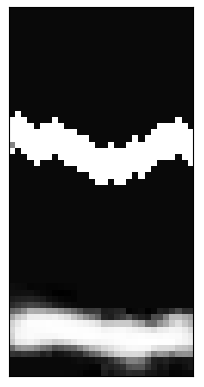
\includegraphics[width=\linewidth]{documentation/report/img/cvae_scroll_tunn.png}
		\caption{Tunnel.}
		\label{subfig:cvae_scroll_tunnel}
	\end{subfigure}

	\caption{Reconstruction of CVAE trained on multiple scroller tasks (Race, Walls Evasion and Tunnel). For each task the ground-truth (upper images) and the reconstructions (lower images) are depicted.}
	\label{fig:cvae_multitask}
\end{figure}

% JANUS MT
\begin{figure}[t!]
	\centering
	\begin{subfigure}{0.3\columnwidth}
		\centering
		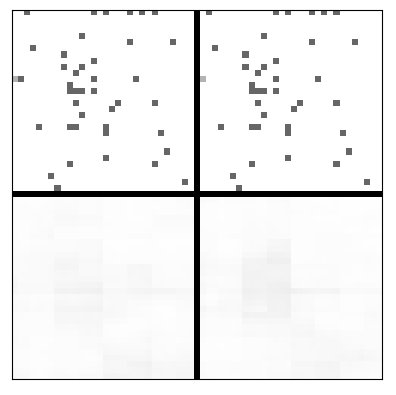
\includegraphics[width=\linewidth]{documentation/report/img/janus_scroll_evasion.png}
		\caption{Evasion.}
		\label{subfig:janus_scroll_race}
	\end{subfigure}%
	~ 
	\begin{subfigure}{0.3\columnwidth}
		\centering
		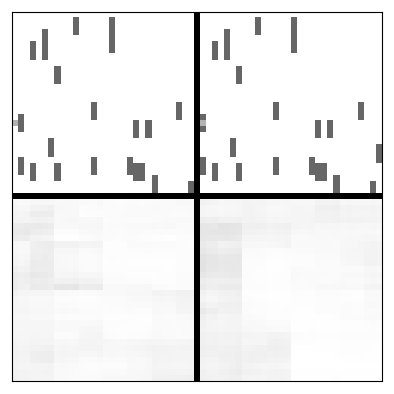
\includegraphics[width=\linewidth]{documentation/report/img/janus_scroll_walls.png}
		\caption{Wall Evasion.}
		\label{subfig:janus_scroll_walls}
	\end{subfigure}%
	~ 
	\begin{subfigure}{0.3\columnwidth}
		\centering
		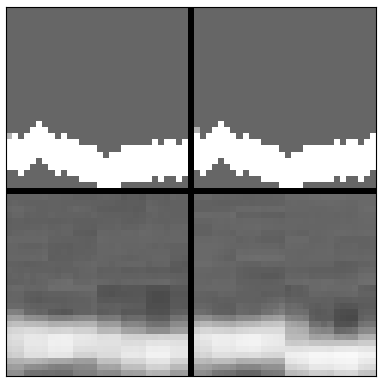
\includegraphics[width=\linewidth]{documentation/report/img/janus_scroll_tunnel.png}
		\caption{Tunnel.}
		\label{subfig:janus_scroll_tunnel}
	\end{subfigure}

	\caption{Reconstruction of Janus trained on multiple scroller tasks (Race, Wall Evasion and Tunnel). For each task the ground-truth (upper images) and the reconstructions (lower images) are depicted.}
	\label{fig:janus_multitask}
\end{figure}


% CERBERUS MT 
\begin{figure}[t!]
	\centering
	\begin{subfigure}{0.3\columnwidth}
		\centering
		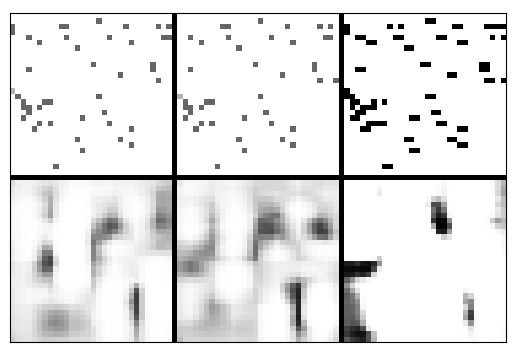
\includegraphics[width=\linewidth]{documentation/report/img/cerb_scroll_evasion.png}
		\caption{Evasion.}
		\label{subfig:cerberus_scroll_race}
	\end{subfigure}%
	~ 
	\begin{subfigure}{0.3\columnwidth}
		\centering
		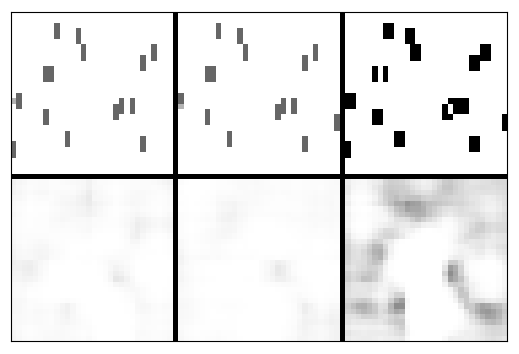
\includegraphics[width=\linewidth]{documentation/report/img/cerb_scroll_walls.png}
		\caption{Wall Evasion.}
		\label{subfig:cerberus_scroll_walls}
	\end{subfigure}
	~ 
	\begin{subfigure}{0.3\columnwidth}
		\centering
		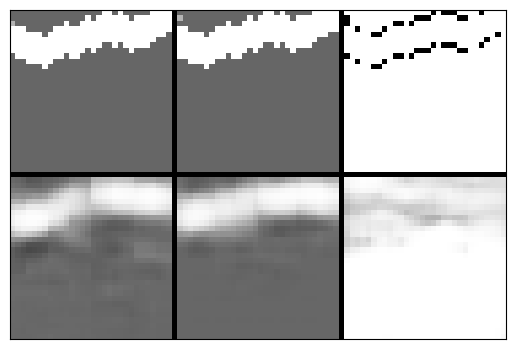
\includegraphics[width=\linewidth]{documentation/report/img/cerb_scroll_tunn.png}
		\caption{Tunnel.}
		\label{subfig:cerberus_scroll_tunnel}
	\end{subfigure}

	\caption{Reconstruction of Cerberus trained on multiple Scroller tasks (Race, Wall Evasion and Tunnel). For each task the ground-truth (upper images) and the reconstructions (lower images) are depicted.}
	\label{fig:cerberus_multitask}
\end{figure}

In Figures \ref{fig:cvae_multitask}, \ref{fig:janus_multitask} and \ref{fig:cerberus_multitask} the performance of CVAE, Janus and Cerberus is shown resulting from a multi-task learning on the Scroller tasks. The added challenge of reconstructing different environments makes the quality of the decoding decrease. For all architectures, the Tunnel is at least placed in the correct parts of the environment. Note though, that this is useless information for the agent, when performing the task since the position of the tunnel is irrelevant for the agent's relative position inside it. The course is rudimentally approximated by CVAE and Cerberus, but Janus experiences even more difficulties with this. The Evasion and Wall Evasion environment are a bigger challenge. This comes unsurprising, since the placement of obstacles is entirely random while the Tunnel forms a continuous entity. Interestingly, the CVAE's reconstructions in these tasks seem to be entirely unrelated to the input. For Evasion, no structure can be observed. The Wall Evasion reconstruction contains structure, but without any obvious connection to the input state. Janus produces reconstructions with slightly more structure than the CVAE Evasion reconstruction for both Evasion and Wall Evasion. Only in the case of Evasion there is a visible connection between the input and output: The area where pixels are densely agglomerated in the input is shaded darker in the reconstruction. Cerberus produces structure with the most contrast in its reconstructions for Evasion and Wall Evasion. For both tasks, the reconstruction is very imprecise, but white areas seem to resemble empty areas of the input.

We attribute the ability of Cerberus to reconstruct sharper edges than Janus to the difference-decoder forcing the reconstruction to pay more attention to the contours.

Due to the undesirable performance of CVAE and the limited computation power, we do not include it in further experiments.
%Since CVAE seems to struggle most with the multi-task setting and our time and computation power resources are limited, we will exclude it from the full system experiments.

\subsubsection{Latent Space Analysis}
\begin{figure}[t!]
	\centering
	\begin{subfigure}{0.46\columnwidth}
		\centering
		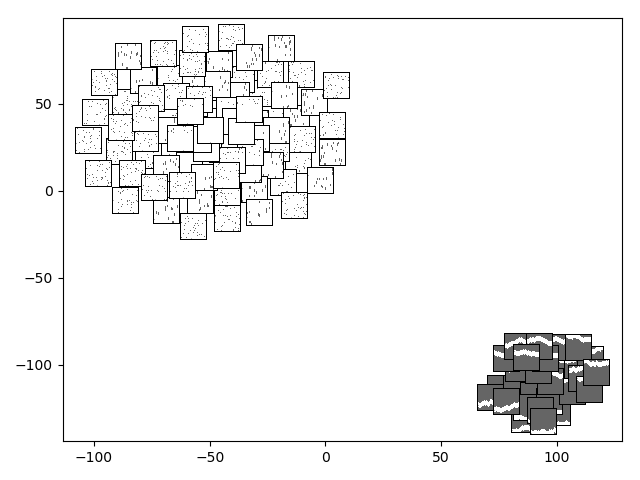
\includegraphics[width=\linewidth]{documentation/report/img/scroller_state.png}
		\caption{t-SNE on raw states.}
		\label{subfig:tsne_multitask_states}
	\end{subfigure}%
	~ 
	\begin{subfigure}{0.46\columnwidth}
		\centering
		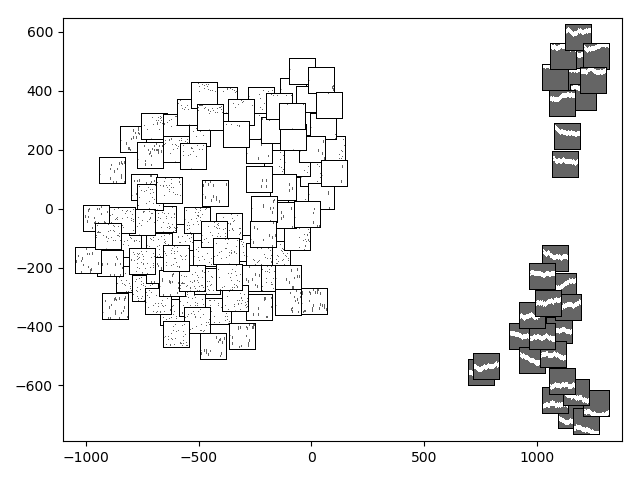
\includegraphics[width=\linewidth]{documentation/report/img/scroller_latent.png}
		\caption{t-SNE on latent states.}
		\label{subfig:tsne_multitask_latent}
	\end{subfigure}

	\caption{t-SNE projections in the multitask environment.}
	\label{fig:tsne-multitask}
\end{figure}

\begin{figure}[t!]
	\centering
	\begin{subfigure}{0.46\columnwidth}
		\centering
		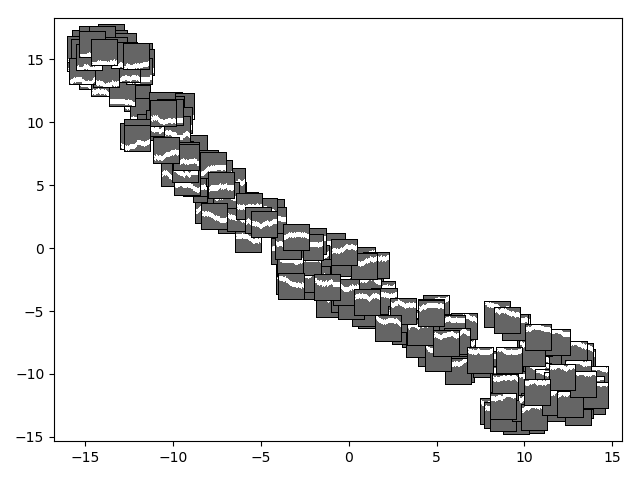
\includegraphics[width=\linewidth]{documentation/report/img/tunnel_state.png}
		\caption{t-SNE on raw states.}
		\label{subfig:tsne_tunnel_states}
	\end{subfigure}%
	~ 
	\begin{subfigure}{0.46\columnwidth}
		\centering
		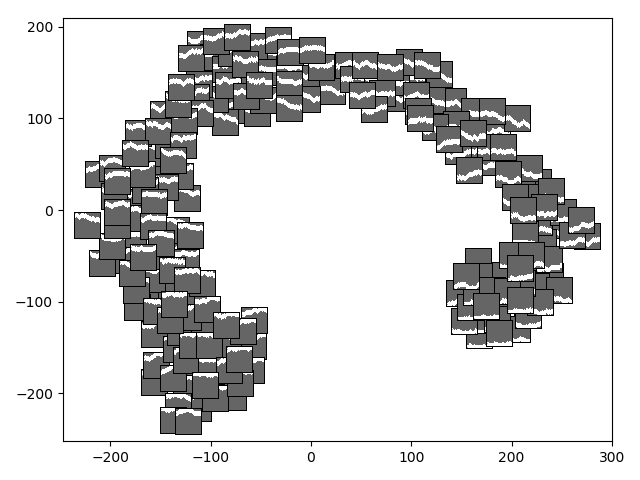
\includegraphics[width=\linewidth]{documentation/report/img/tunnel_latent.png}
		\caption{t-SNE on latent states.}
		\label{subfig:tsne_tunnel_latent}
	\end{subfigure}

	\caption{t-SNE projections in the Tunnel environment.}
	\label{fig:tsne-tunnel}
\end{figure}

To inspect the latent representations constructed by the encoders, we visualize the encoded states from different tasks with t-Distributed Stochastic Neighbor Embedding (t-SNE) \citep{tsne}. 

\paragraph{Latent Space of Multiple Tasks}
Figure \ref{fig:tsne-multitask} shows the original states and the latent states respectively with their dimensionalities reduced to two. Thirty states are sampled from each of Evasion, Wall Evasions, and Tunnel. 
As t-SNE preserves relative distances in high dimensional spaces, the frames closer to each other in the visualizations tend to be closer in the original spaces too.

In Figure \ref{subfig:tsne_multitask_states}, the original 30*30 input are plotted on two dimensions.
As expected, frames from Tunnel form their own cluster far apart from those from other tasks due to their distinct spatial characteristic, namely the large continuous areas of dark pixels. One can further observe that the nearly-empty frames are closer to each other, forming the center of the lower-left cluster.
This center is surrounded by other frames containing more dark pixels.

The t-SNE output in Figure \ref{subfig:tsne_multitask_latent} is based on the encoded latent states, although only the original frames are plotted to aid visual interpretation.
Unlike previously, the embedding clearly distinguishes the frames with dense dark pixels from those without. It furthermore shows a smooth gradient corresponding to the change in dark pixel density.
This provides evidence that the latent representation is able to capture abstract features of the inputs.
However, the frames from Tunnel still fall far from the other tasks, indicating that the encoder has not found a common representation for all tasks.
It is also visible that there is a further separation of Tunnel frames based on their spatial arrangements, i.e. the positions of the tunnels.

\paragraph{Latent Space of Tunnel Task} \label{para:latent_tunnel}
When using the representation module trained only on Tunnel and projecting latent spaces from Tunnel using t-SNE (Figure \ref{fig:tsne-tunnel}), a key problem of our approach becomes apparent. 
The additional structure in the Tunnel environment reveals the encoders inability to identify information relevant to tasks, that is, local information around the agent for these tasks. 
%Instead, the latent space is separating based on general structure.
Instead, the latent space is constructed based on the spatial structure of the frame, that is, the positions of the tunnel.
%In the case of the tunnel frames, this shows in the position of the tunnel in the frame being indicative of the latent space distance between states. 
As Figure \ref{subfig:tsne_tunnel_states} shows, this is the case without any latent state transformation as well. 

The curved structure in Figure \ref{subfig:tsne_tunnel_latent} could indicate that the latent space finds similarities between frames that would be more similar when horizontally mirrored.
However, this information is not useful for the agent when learning the task. In fact, the latent space should be grouping the frames based on the course of the tunnel and the current position of the agent. 

\subsection{Policy Learner}
The results for the different tasks were taken from a point during a 50,000 episode training where intermediate performance was maximal. This avoids taking the policy in a state where the agent currently reconsiders its solution to potentially find a better one.

Table \ref{tab:isolated_policy_learner} shows the performance of the DDQN on four tasks respectively. 
Note that the autoencoder weights are not updated by its own loss in order to test the policy learner in isolation.
On Pathing, Race, and Evasion, the performance is close to maximal and significantly outperform the random baselines.
However, in the Tunnel task the DDQN fails to learn an effective policy.
Its resulting behavior is simply a straight horizontal movement without any action initiated by the agent itself.

Since the effectiveness of the policy learner is proven on other tasks, we hypothesize that the poor performance is due to the latent representation not capturing useful information for this particular task.
The previous analysis of the latent space structure in Section \ref{para:latent_tunnel} provides further support for this hypothesis.
As previously stated, Figure \ref{subfig:tsne_tunnel_latent} shows that the latent representations for horizontally mirrored states are closer to each other. 
This contradicts the intuition that the learned representation should capture information about edge avoidance and therefore place such frames far apart.
%The fact that even the original DDQN without our modification cannot learn to do this trained on Tunnel alone (compare Table \ref{tab:isolated_policy_learner}) indicates the challenges posed by this task. 
But this observation also underlines the general difficulty of balancing between focusing on task-relevant features and generalizing for transfer learning.


\begin{table}[t!]
\centering
\begin{tabular}{@{}lllll@{}}
\toprule
\textbf{Task} & \textbf{$\mu_r$} & \textbf{$\widetilde{r}$} & \textbf{$\sigma_r$} & \textbf{baseline} \textbf{$\mu(r)$} \\ \midrule
Pathing & $-480$ & $-480$ & $0$ & $-8988$ \\
Race & $4103.6$ & $5000$ & $1783.8$ & $472$ \\
Evasion & $3949.7$ & $5000$ & $1543.7$ & $487.89$ \\
Tunnel & $193$ & $140$ & $313.06$ & $120$\\ 
\bottomrule
\end{tabular}
\caption{Performance of the DDQN without autoencoder loss but using a convolutional encoder. Results are given as arithmetic mean $\mu_r$ and median $\widetilde{r}$ over 100 test episodes. Baselines are random policies and therefore the absolute minimum performance. For the Race, Evasion and Tunnel task, maximum performance is 5000, while for Pathing -480 is the best score achievable.}
\label{tab:isolated_policy_learner}
\end{table}

% FINAL TEST ON TRANSFER
\subsection{Full System Experiments}
After performing individual experiments over the modules, we decided to not include the Convolutional Variational Autoencoder in the final experiments, being the representation module that performed worse, especially in a multi-task context.

\subsubsection{Zero-shot}
In Table \ref{zero-shot-table} are depicted statistics concerning different training configurations.
All results of this section are calculated over $10000$ test-runs and include average, peak and median reward.

The zero-shot experiment showed no visible gain in using the pre-trained model. In fact, the collected reward of the pre-trained architectures was as inefficient as the random initialization, showing no valuable knowledge transfer.

\begin{table}[t!]
\begin{tabular}{llllll}
\toprule
pre-training   & $\mu_r$ & max $r$ & $\widetilde{r}$ \\ \midrule
Random Initialization                           &     $481.22$     &    $2260$     &      $420$      \\ \midrule
Janus Scrollers &     $479.46$     &    $2210$     &      $420$      \\ 
Cerberus Scrollers &     $479.06$     &    $2080$     &      $420$      \\ \midrule 
Janus Tunnel    &     $477.55$     &    $2620$     &      $420$      \\ 
Cerberus Tunnel    &     $481.00$     &    $2530$     &      $420$      \\ \bottomrule 

\end{tabular}
\caption{Zero-Shot performance of proposed architectures compared with untrained agent on task Race. All pre-trainings trained on ~900,000 episodes. Statistics were calculated on 10,000 testruns.}
\label{zero-shot-table}
\end{table}

\subsubsection{Improved Learning from Transfer}

In Figure \ref{fig:improved-learning} is depicted the collected reward of the system when pre-trained on the Tunnel task and on the Scroller tasks compared to the untrained model.
As the graph clearly shows, the system was not able to learn any interesting policy when trained starting from a pre-trained model, and the only configuration that managed to learn a correct policy - getting the max reward in several occasions - was the untrained one.

\begin{figure}
    \centering
    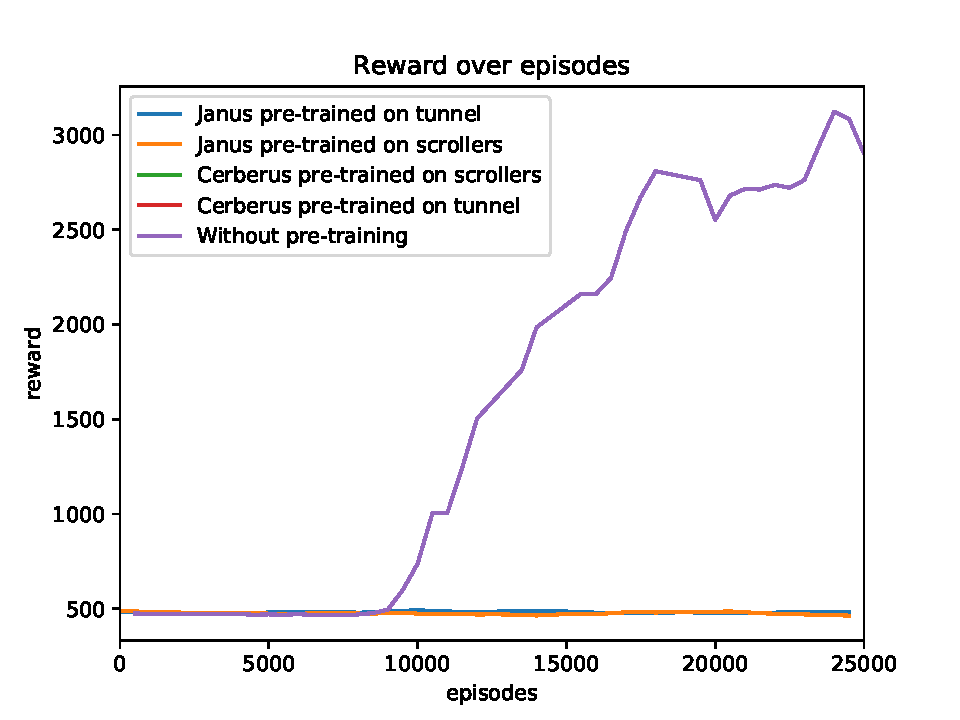
\includegraphics[width=\columnwidth]{img/rewards.pdf}
    \caption{Development of average rewards when training an agent for the Race task with either random initialization or pre-trained on Tunnel/Scrollers using Janus/Cerberus.}
    \label{fig:improved-learning}
\end{figure}